%%%%%%%%%%%%%%%%%%%%%%%%%%%%%%%%%%%%%%%%%%%%%%%%%%%%%%%%%%%%%%%%%%%%%%
% Overleaf (WriteLaTeX) Example: Molecular Chemistry Presentation
%
% Source: http://www.overleaf.com
%
% In these slides we show how Overleaf can be used with standard 
% chemistry packages to easily create professional presentations.
% 
% Feel free to distribute this example, but please keep the referral
% to overleaf.com
% 
%%%%%%%%%%%%%%%%%%%%%%%%%%%%%%%%%%%%%%%%%%%%%%%%%%%%%%%%%%%%%%%%%%%%%%
% How to use Overleaf: 
%
% You edit the source code here on the left, and the preview on the
% right shows you the result within a few seconds.
%
% Bookmark this page and share the URL with your co-authors. They can
% edit at the same time!
%
% You can upload figures, bibliographies, custom classes and
% styles using the files menu.
%
% If you're new to LaTeX, the wikibook is a great place to start:
% http://en.wikibooks.org/wiki/LaTeX
%
%%%%%%%%%%%%%%%%%%%%%%%%%%%%%%%%%%%%%%%%%%%%%%%%%%%%%%%%%%%%%%%%%%%%%%

\documentclass{beamer}

% For more themes, color themes and font themes, see:
% http://deic.uab.es/~i %lanes/beamer_gallery/index_by_theme.html
%
\mode<presentation>
{
  \usetheme{CambridgeUS}       % or try default, Darmstadt, Warsaw, ...
  \usecolortheme{whale} % or try albatross, beaver, crane, ...
  \usefonttheme{default}    % or try default, structurebold, ...
  \setbeamertemplate{navigation symbols}{}
  \setbeamertemplate{caption}[numbered]
  \setbeamerfont{frametitle}{size=\footnotesize}
  \setbeamertemplate{bibliography item}[text]
} 

\usepackage[english]{babel}
\usepackage[utf8x]{inputenc}
\usepackage{multicol}
\usepackage{caption}

% Here's where the presentation starts, with the info for the title slide
\title[Muon Rate - Phys 314]{Temperature (Time?) Variation in Muon Detection Rate}
\author[Ian Hunt-Isaak]{Ian Hunt-Isaak}
\institute[Oberlin College]{Partner: Corina Miner}
\date{December 10, 2015}

\begin{document}

\begin{frame}
  \titlepage
\end{frame}

% These three lines create an automatically generated table of contents.
%\begin{frame}{Outline}
%  \tableofcontents
%\end{frame}

\section{Introduction}
\subsection{Theory}
\begin{frame}{Muon Sources}
\begin{itemize}
	\item Cosmic Rays $\to$ Muons
	\item Sun Cosmic Rays $\to$ Day/Night rate variation?
\end{itemize}
\begin{center}
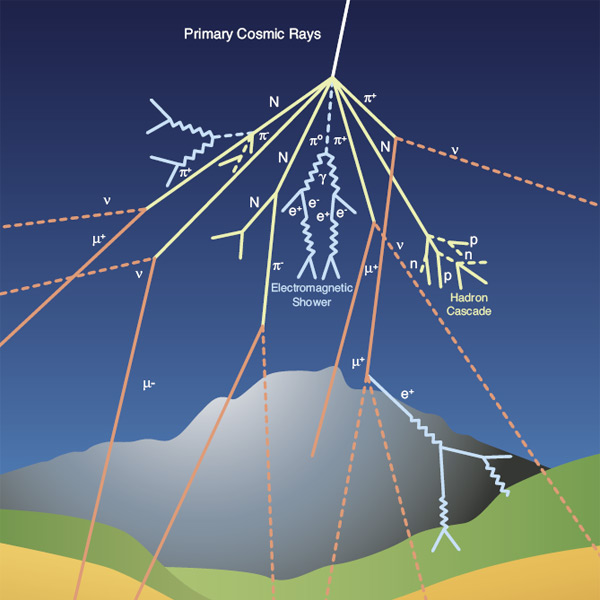
\includegraphics[scale=.25]{../Figures/cosmic_ray.jpg}
\hspace{20pt}
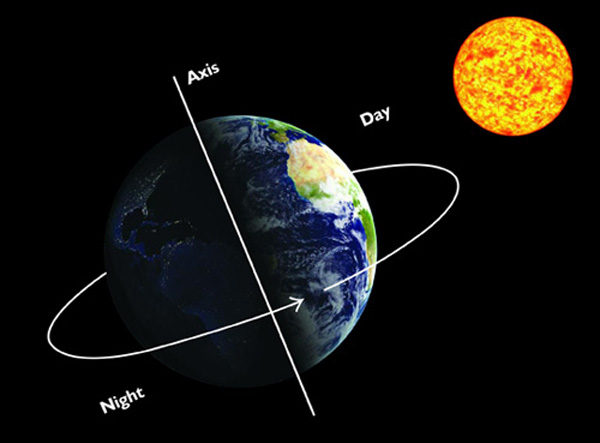
\includegraphics[scale=.25]{../Figures/dayNight.jpg}
\end{center}
\end{frame}


\begin{frame}{Confounding Effects}
\begin{itemize}
	\item Temperature affecting Detector
	\item Solar Activity
\end{itemize}
\end{frame}

\subsection{Experimental Setup}

\begin{frame}{Experimental Setup}
\centering
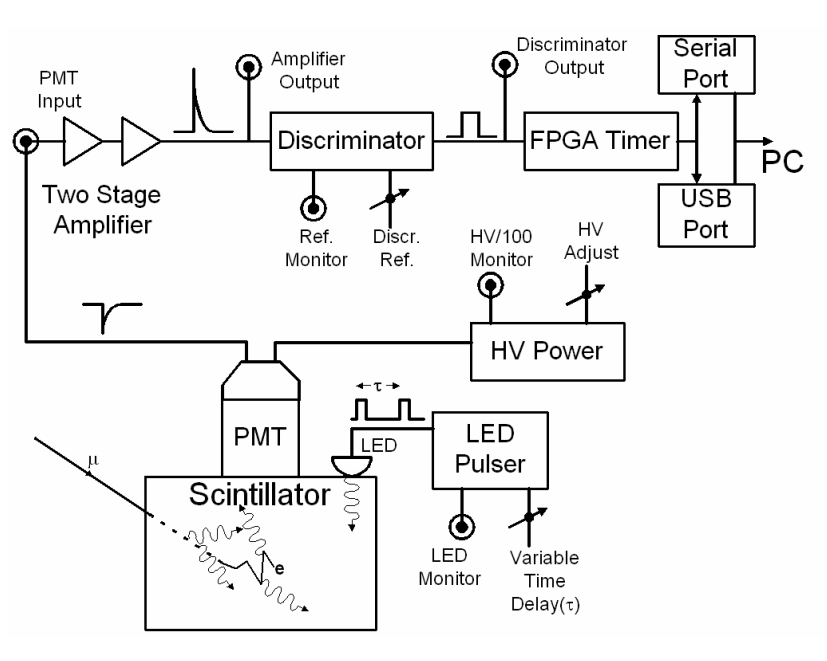
\includegraphics[scale=.25]{../Figures/MuonBlockDiagram.png}
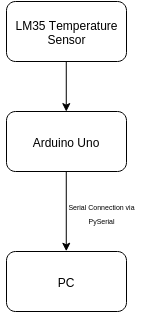
\includegraphics[scale=.5]{../Figures/temperatureBlockDiagram.png}\\
\tiny{Left Diagram from \cite{muonPhysics}}


\end{frame}


\section{Results - Analysis}

\subsection{Temperature Variation}

\begin{frame}{Results - Hourly Temperature Variation}
\begin{center}
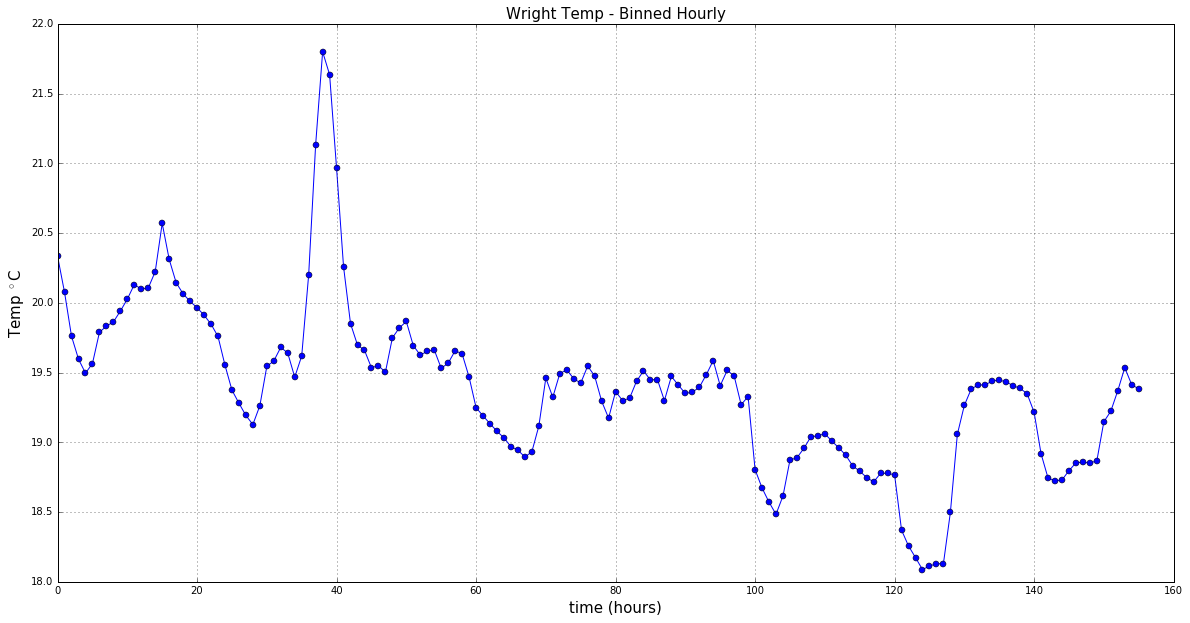
\includegraphics[scale=.25]{../Figures/tempVariation-Wide.png}
\end{center}
\end{frame}


\begin{frame}{Hourly Temperature Variation with Muon Rate}
\begin{center}
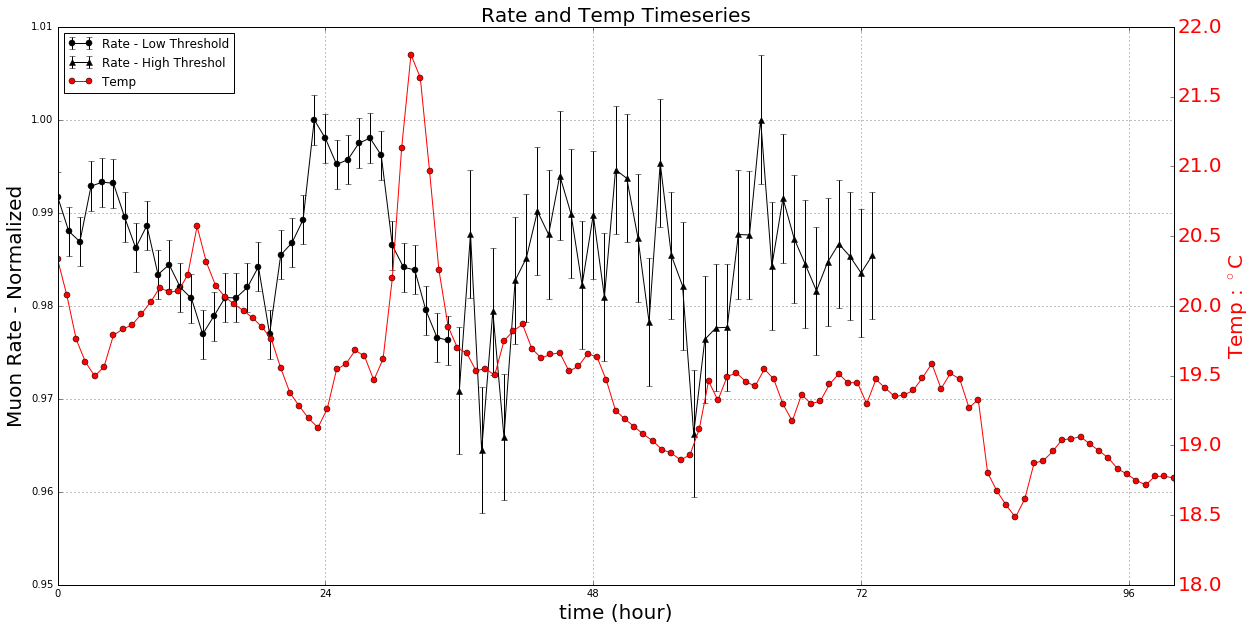
\includegraphics[scale=.27]{../Figures/bothTempVariation-Wide.png}
\end{center}
\end{frame}

\begin{frame}{Temperature Rate Correlation}
\centering

\small{
\begin{center}
	\begin{tabular}{|c|c|c|}\hline
		Data Set & Slope & $\tilde{\chi}^2$ \\ \hline\hline
		Low Threshold& $-0.0114 \pm 0.0028 $ & 4.681  \\ \hline
		High Threshold &$-0.0053 \pm 0.0017 $ & 1.099\\ \hline
	\end{tabular}
\end{center}
}

\begin{figure}
\begin{multicols}{2}
\centering
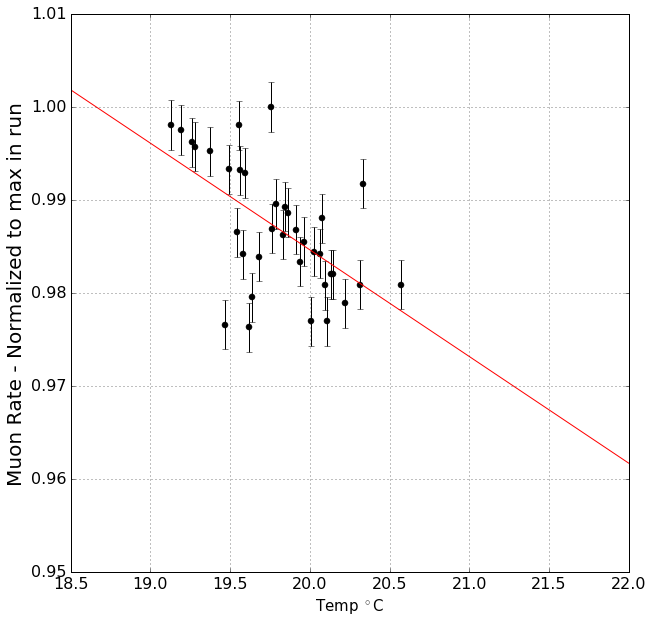
\includegraphics[scale=.22]{../Figures/lowCorrelation.png}\\
$200$ mV Threshold
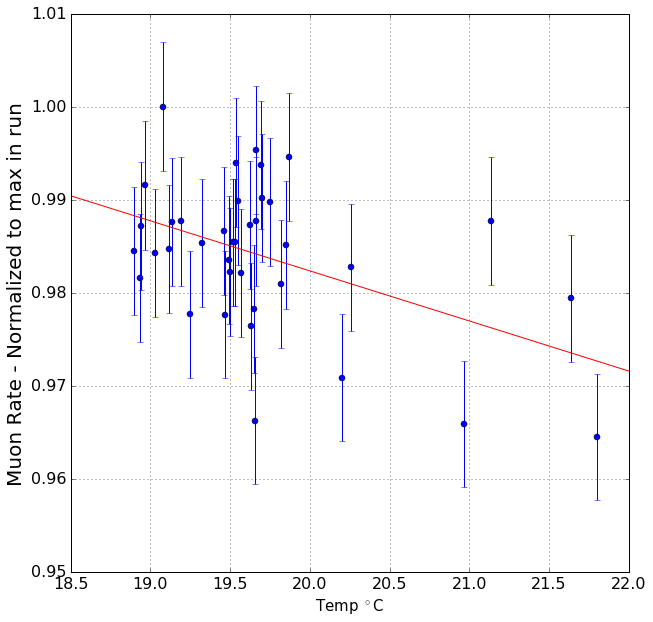
\includegraphics[scale=.22]{../Figures/highCorrelation.png}\\
$400$ mV Threshold
\end{multicols}
\vspace {0pt}
%\setlength{\abovefigureskip}{-30pt}
{\caption*{}}
\end{figure}

\end{frame}


\begin{frame}{Possible Explanations}
	\begin{itemize}
	\item Threshold voltage drift
	\item Photomultiplier Gain
	\item Electronics Efficiency
	\item Noise
	\item Muons only come inside when its cold out
	\end{itemize}
\end{frame}


\section{Next Steps\dots{}}

\begin{frame}{Next Steps\dots{}}

\begin{itemize}
\item Fix Muon Rate Data collection
\item Record Threshold voltage to try to detect drift
\item Correct for temperature offset
\item Better Data $\to$ More Complicated Temperature Dependence
\end{itemize}


\end{frame}
\begin{frame}
\begin{thebibliography}{9}
\bibitem{muonPhysics}
	T.E Coan, J. Ye,
	\emph{Muon Physics},
	Accessed from Blackboard site
\bibitem{stalknaker}
	J. Stalnaker, Personal Correspondence
\bibitem{muonRate}
	N. Ramesh, M. Hawron, C. Martin, A. Bachiri,
	\emph{Flux Variation of Cosmic Muons}
	arxiv.org/pdf/1203.0101.pdf
\bibitem{rotationPic}
	Accessed from \url{http://i.cdn-surfline.com/forecasters/blog/2013/12_dec/121813_3.jpg}


\end{thebibliography}
\end{frame}

\end{document}